\chapter{nginx}
\label{ch:nginx}

\section{Introduction}

The context of this project is to implement a testbed for a \textit{\gls{toe}} being developed in another research project. This testbed should enable testing the \gls{toe} in an environment and with workloads close to usage in real world. One usage of \gls{tcp} is as transport layer for \gls{http} requests. \gls{http} is the second most used protocol among all internet traffic, with a share of about 20 to 30 \% (in 2008/09) \cite{internet_study} and therefore very relevant outside of lab environments. 

The server-side endpoint for \gls{http} traffic is a web server software. For this project \textit{nginx} (pronounced "engine-x") was chosen, which follows an asynchronous architecture. It was released to the public in 2004 and focuses on "high performance, high concurrency and high memory usages" \cite{aosa}. Creator and main developer of nginx is Igor Sysoev\footnote{\url{http://sysoev.ru/en/}}.

A server system, like a web server, needs to be non-blocking to handle multiple requests at once. That is it must be able to accept and process requests while it is still busy with other, previously received requests. Systems with a "traditional" (i.e. thread-based) architecture fulfill this requirement by spawning separate processes or threads for incoming requests. An application designed by this model does not favor performance, because spawning new processes or threads "requires preparation of a new runtime environment, including allocation of heap and stack memory, and the creation of a new execution context" \cite{aosa}.

In contrast to this, \textit{nginx} was designed following in an asynchronous architecture, which is accomplished by using a so called event-pattern. This means -- very much simplified -- that \textit{nginx} never "waits" during processing a request for any external operation to complete, but pushes it to an event system, being part of the \gls{os}, does something other useful like processing new requests and picks up the event, when it is finished for further processing steps.

\section{Architecture}
\label{sec:nginx-arch}

\subsection{Overview}

A running \textit{nginx} instance always consists of atleast two processes: a \textbf{master} and a \textbf{worker} process. The master process spins-up, monitors and controls the worker processes. The worker processes process the actual (HTTP) requests on a single thread.

%\setlength{\intextsep}{0pt}
\begin{wrapfigure}[12]{r}{.4\textwidth}
	\centering
	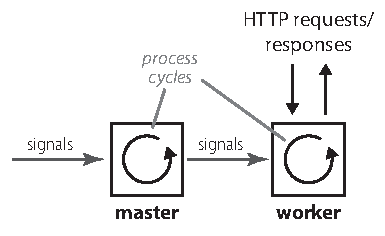
\includegraphics[scale=1]{images/nginx-overview.pdf}
	\caption{Overview of nginx process model.}
	\label{fig:nginx-overview}
\end{wrapfigure}

After initialization both processes run in a so called \textbf{process cycle}. That is an infinite loop with the process waiting to be activated from suspension by external events. For the master process these are signals send to the process which might indicate requests for shutdown, configuration reload or previously initiated timed events.

Design of the worker process had as key principle "to be as non-blocking as possible" \cite{aosa}. This is done by relying heavily on asynchronous operations being implemented through "modularity, event notifications, extensive use of callback functions and fine-tuned timers" \cite{aosa}. It also makes the process cycle of the worker process the "most complicated part of \textit{nginx}" \cite{aosa}.

Processing of requests is outsourced from the \textit{nginx} core routines to a number of dedicated modules. These modules hook into a processing pipeline forming a \textbf{chain of modules}. When a request receives, it is passed through the pipeline with every module doing the relevant work \cite{aosa}. Functionality of modules includes handling a specific protocol (e.g. \gls{http}), modifying content, filtering, handling special variables or load balancing. It is also possible to develop and integrate custom modules.

An \gls{http} request runs through a number of processing phases with dedicated \textbf{phase handlers}. These process a request and generate an appropriate response, send the header and send the body. Generation of content is done by \textbf{content handlers}. Out-of-the-box there exist several default handlers for index views or simple static files. The result of this handlers is passed to \textbf{filters} performing outbound content modifications. Filters form a separate processing pipeline, passing results among themselves until the final filter is called. Functionality of filters includes amongst others generation of header data, charset modification and gzip compression. \cite{aosa}

\subsection{Event-driven Architecture}

Another task of modules in the \textit{nginx} architecture is to implement functionality specific to a certain \gls{os}. One of this specifically designed tasks is the integration of an event module. Consistent and strict usage of the event-driven architecture is the fundamental point of \textit{nginx}.

This is accomplished by using asynchronous, i.e. non-blocking, i/o-functions of the operating system. Handling of returning events is done through an event module provided by the \gls{os}. For this project Linux's \textit{epoll}\footnote{\url{http://linux.die.net/man/4/epoll}} module is used. \textit{epoll} handles events on file descriptors. Therefore also network related and custom events can be handled, because in Linux everything is a file descriptor\footnote{Linus Torvalds, "The everything-is-a-file principle": \url{http://yarchive.net/comp/linux/everything_is_file.html} (as of 12/2012)} (or process).

Events are queued and dequeued in the worker process cycle. The total workload for processing a request is split into multiple chunks, each handled when necessary operations of the \gls{os} returned.

\begin{figure}[H]
	\centering
	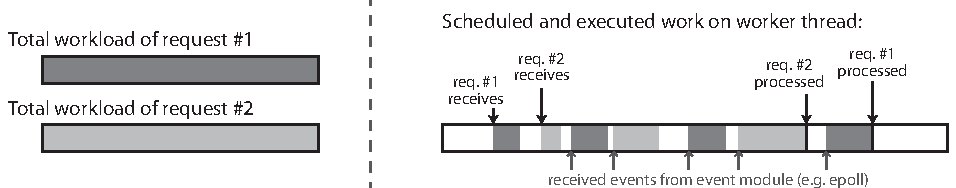
\includegraphics[scale=1]{images/nginx-event-proc.pdf}
	\caption{Processing model of worker threads.}
	\label{fig:nginx-event-proc}
\end{figure}

This leads to a responsive nginx worker thread which "can handle many thousands of concurrent connections and requests per second" (on a decent server system) \cite{aosa}.

\section{Configuration and Building}
\label{sec:nginx-config}

After this general overview of \textit{nginx}'s architecture and underlying concepts, the next section focuses on practical implications of bringing \textit{nginx} to a \textit{MicroBlaze} system.

\subsection{Extending the Configuration System}

The build process of \textit{nginx} can be configured with a number of parameters and constants to add or remove optional modules. The inclusion of modules can be configured with command line arguments to the configuration tool, but many of the parameters can not be set externally.

The values of these parameters are determined by a custom "auto configuration" tool. This tool writes small c programs to a temporary file, compiles them using the configured compiler and reads back the results. By this process \textit{nginx} adjusts its own build process to the features and properties of the current system. This configuration process is not working for cross-compiling \textit{nginx} for another target system. Therefore the configuration process needed to be extended to allow input of required configuration parameters into the build process from an external source.

The implemented solution is based on a suggested patch by Daniele Salvatore Albano\footnote{\textit{Cross compilation support for nginx}, Daniele Salvatore Albano, 01/03/2011 \url{http://web.archiveorange.com/archive/v/Tuw7Ryz8rztiNaIFfqCg}}, but incorporates more parameters and is streamlined to the process of cross-compiling the Linux kernel. Cross-compiling can be enabled by setting the environment variable "\texttt{CROSS\_COMPILE}" to the suitable compiler tool chain prefix. For the \textit{MicroBlaze} tool chain this is "\texttt{microblaze-unknown-linux-gnu-}".

Parameters that are covered by this modification to the configuration system include endianness (\texttt{with-endian}), the size of primitive data types (\texttt{with-int}, \texttt{with-long}, etc.) and the maximum error number, to be used for custom error types (\texttt{with-sys-nerr}).

Value for these introduced parameters can be determined through a small test program executed on the \gls{soc} (see appendix \ref{sec:nginx-env-eval}). This leads to the following values:

\begin{verbatim}
    --with-endian=big \
    --with-sys-nerr=132 \
    --with-int=4 \
    --with-long=4 \
    --with-long-long=8 \
    --with-ptr-size=4 \
    --with-sig-atomic-t=4 \
    --with-size-t=4 \
    --with-off-t=4 \
    --with-time-t=4
\end{verbatim}

\subsection{Modules}

\textit{nginx} consists of a number of (optional) modules. These modules can be in- or excluded from the build using parameters to the configuration tool. Objective of the \textit{nginx} build for the MicroBlaze system was a small binary with just the necessary parts included. There for the following modules were excluded:

\begin{verbatim}
    --without-http_rewrite_module \
    --without-http_gzip_module \
    --without-http_charset_module \
    --without-http_ssi_module \
    --without-http_userid_module \
    --without-http_access_module \
    --without-http_auth_basic_module \
    --without-http_autoindex_module \
    --without-http_status_module \
    --without-http_geo_module \
    --without-http_map_module \
    --without-http_split_clients_module \
    --without-http_referer_module \
    --without-http_proxy_module \
    --without-http_fastcgi_module \
    --without-http_uwsgi_module \
    --without-http_scgi_module \
    --without-http_memcached_module \
    --without-http_limit_conn_module \
    --without-http_limit_req_module \
    --without-http_empty_gif_module \
    --without-http_browser_module \
    --without-http_upstream_ip_hash_module \
    --without-http_upstream_least_conn_module \
    --without-http_upstream_keepalive_module \
    --without-http-cache \
    --without-pcre \
    --without-select_module \
    --without-poll_module
\end{verbatim}

Some of these modules could be included in the build, if necessary, but the modules \texttt{http\_rewrite\_module} and \texttt{http\_gzip\_module} require external libraries which are not present on the MicroBlaze system and therefore would not work.

\subsection{Compiler Configuration}

Besides the configuration for \textit{nginx} itself, the compiler needs to be configured for the target MicroBlaze system. When building the Linux kernel, the compiler configuration is set by the configuration of the kernel during the build process. \textit{nginx} does not have this functionality in its configuration system, but comes with a parameter (\texttt{--with-cc-opt=...}) to pass custom parameters to the compiler.

Through this configuration setting, the gcc cross-compiler needs to be configured for the feature set of the MicroBlaze system. For the presented MicroBlaze \gls{soc}, the required parameters are

\texttt{-mxl-multiply-high -mno-xl-soft-mul -mno-xl-soft-div} $\hookleftarrow$ \\
\texttt{-mxl-barrel-shift -mxl-pattern-compare -mcpu=v8.30.a}

Additionally the path to the standard libraries on the system needs to be set through the \texttt{--sysroot} parameter. These libraries are part of the tool chain for \textit{MicroBlaze} systems provided by \textit{Xilinx}. 

By specifying the \texttt{----static} parameter all referenced libraries are build into the resulting binary. Therefore the binary has less dependencies to be executed.

Combining it all together the value of the \texttt{--with-cc-opt} parameter needs to be set to something like the following: 

\texttt{--with-cc-opt="-mxl-multiply-high -mno-xl-soft-mul -mno-xl-soft-div} $ \hookleftarrow$ \\
\texttt{-mxl-barrel-shift -mxl-pattern-compare -mcpu=v8.30.a ----static} $ \hookleftarrow$ \\
\texttt{----sysroot=/home/peschuster/project/microblaze-unknown-linux-gnu/} $ \hookleftarrow$ \\
\texttt{microblaze-unknown-linux-gnu/sys-root"}

\subsection{Memory Leaks}

One problem that arose during tests were memory leaks. It turned out that \textit{nginx} allocated about 4053.2 Bytes of memory for each request. Assuming available memory of about 200 MB, \textit{nginx} crashed the complete system after approximately 50,500 requests in total. of course, this is an unacceptable behavior for a (web) server system.

\begin{figure}[H]
\begin{minipage}{0.4\textwidth}
\begin{tabular}{|r|r|r|}
    \hline
     \textbf{requests} & \textbf{master / KB} & \textbf{worker / KB} \\
    \hline
    0     & 3064  & 3204 \\
    1000  & 3064  & 7296 \\
    2000  & 3064  & 11256 \\
    3000  & 3064  & 15348 \\
    4000  & 3064  & 19440 \\
    5000  & 3064  & 23404 \\
    6000  & 3064  & 27496 \\
    7000  & 3064  & 31588 \\
    8000  & 3064  & 35552 \\
    9000  & 3064  & 39644 \\
    10000 & 3064  & 43736 \\
    \hline
    \end{tabular}
\end{minipage}
\begin{minipage}{0.60\textwidth}
	\centering
	\begin{tikzpicture}
		\begin{axis}[width=\textwidth,height=7cm,
			xlabel={requests},
			ylabel={memory / KB},
			xmin=0,
			ymin=0,
			xmax=10000,
			extra y ticks={3064},
			%extra y tick label style={/pgf/number format/1000 sep=},
			extra y tick style={grid=major},
			extra x tick style={grid=major},
			y tick label style={/pgf/number format/1000 sep=},
			legend pos = north west]
			\addplot table[x index=0, y index=1] {graphdata/nginx-mem.csv};
			\addlegendentry{master process}
			\addplot table[x index=0, y index=2] {graphdata/nginx-mem.csv};
			\addlegendentry{worker process}
		\end{axis}
	\end{tikzpicture}
\end{minipage}
  \caption{Memory consumption of nginx processes over total requests.}
  \label{fig:nginx-mem}
\end{figure}

\subsubsection{Investigations}

The described behavior of \textit{nginx} could not be replicated on a standard x86 server system running \textit{Ubuntu Linux 12.04}. That means \textit{nginx} in general should work correct, using just as much memory as required and releasing unused memory to the \gls{os}. However, on the \textit{MicroBlaze} system this does not work properly.

With activated \texttt{debug} log. \textit{nginx} writes some information about inner workings to the error log. The debug log can be activated with the following option in the configuration file:

\begin{verbatim}
error_log  logs/error.log  debug;
\end{verbatim}

There must be only one \texttt{error\_log} line in the \textit{nginx} configuration file, but the option specifying the severity level is inclusive for all lower levels.

The following table shows all memory related debug messages as found in the error log for a single request to a static file on the \textit{MicroBlaze} system running a \textit{nginx} instance, which is configured as described in the previous section (\ref{sec:nginx-config}):

\begin{table}[H]
\centering
\begin{tabular}{|l|l|r|r|}
    \hline
     \textbf{Log entry} & \textbf{ptr} & \textbf{allocated} & \textbf{freed} \\
    \hline \hline
\texttt{*1 malloc: 10080890:644} & 10080890 & 644 &  \\ \hline
\texttt{*1 malloc: 10080B18:1024} & 10080B18 & 1024 &  \\ \hline
\texttt{*1 posix\_memalign: 1007B5B0:4096 @16} & 1007B5B0 & 4096 &  \\ \hline \hline
\texttt{*1 free: 1007B5B0, unused: 2079} & 1007B5B0 & & 4096 \\ \hline
\texttt{*1 free: 10080890} & 10080890 & & 644 \\ \hline
\texttt{*1 free: 10080B18} & 10080B18 & & 1024 \\ \hline
\end{tabular}
\caption{Memory management related debug messages of a single request.}
\label{tab:debug_mem}
\end{table}

All pointers to allocated memory for one request are passed to the \texttt{free(..)} function of the \textit{C Standard Library} (\textit{libc}) and therefore should be released to the system. But performance and stress tests on the system proved a different behavior: The \textit{nginx} worker process consumes more memory for each request with a linear relation to the number of requests (see \ref{fig:nginx-mem}).

Therefore the error causing this misbehavior probably is not located in \textit{nginx} itself, but in the underlying system layers. This would mean that memory management of the Linux kernel or \textit{libc} port to the \textit{MicroBlaze} architecture are broken, in the described respect. This is a strong allegation, especially because fully analyzing the problem on this wide dimensions was beyond the scope of this bachelor thesis. But there are a view points promoting this theory which should be considered:

There is an answer by \textit{Xilinx} support (\textit{AR \#12421}) stating that memory management (especially the function \textit{free(..)}) is "very system-specific" and not fully implemented/supported for \textit{MicroBlaze} processors \cite{mbfree}. The answer was published on 09/09/2010 and is explicitly only valid for versions of the \textit{MicroBlaze} processors without a hardware memory management unit. Therefore it should not apply to the used version of the \textit{MicroBlaze} processor and \textit{C Standard Library}, but it shows that these memory management functions were added to the toolchain and supporting environment only recently and might not be as stable as other parts.

Another point benefiting this theory is the unusual way \textit{nginx} deals with memory. Memory management is done by \textit{nginx}'s pool allocator. This could be seen as an abstraction to the memory allocation mechanisms provided by the \gls{os}. When a module/sub-routine/function requires dynamically allocated memory, it requests it from the \textit{nginx} pool allocator, which itself requests a larger chunk of memory (called "pool") from the \gls{os} and distributes small blocks of the pool on requests from other parts of \textit{nginx}. When no blocks of a pool are used anymore, it is returned to the \gls{os}. \textit{nginx} uses this design to minimize system calls and reduce expensive requests for memory allocation by the hardware memory management unit \cite{aosa}. Another consequence of this design is that \textit{nginx} does not reuse once allocated memory, but just allocates new memory blocks when required and releasing them to the system upon finished operations. This is by design and beneficial for speed and efficiency, but comes in unfavorable, when the memory management of the system (\gls{os} and processor) might not work properly.

\subsubsection{A First Workaround}

It was not possible to fix the root cause of the memory leaks during this bachelor thesis. To circumvent the described arising problems, another solution needed to be found to be able to use the system and conduct extensive performance tests.

A workaround to circumvent complete system crashes during tests due to exhausted memory is to restart the \textit{nginx} worker process on low remaining system memory.

This can be accomplished by sending the \texttt{HUB} signal to the \textit{nginx} master process using the \texttt{kill} command of \textit{Unix} systems\footnote{\url{http://unixhelp.ed.ac.uk/CGI/man-cgi?kill}}. The \texttt{HUB} signal tells \textit{nginx} to reload the current configuration, resulting in spinning up new worker processes and gracefully shutting down the previous ones. This differs from complete restarts of \textit{nginx} in the way that no incoming requests are lost during the restart process\footnote{\url{http://wiki.nginx.org/CommandLine} (as of 12/2012)}.

The process id of the master process on the system under test is always stored in the file \texttt{/usr/local/nginx/logs/nginx.pid}. Therefore the complete command for restarting the \textit{nginx} worker process can be constructed as follows:

\begin{verbatim}
kill -HUP $( cat /usr/local/nginx/logs/nginx.pid )
\end{verbatim}

Information about currently allocated and free memory can be displayed using tools like \textit{top}\footnote{\url{http://www.busybox.net/downloads/BusyBox.html\#top}}, which provide "a view of process activity in real time" \cite{busybox}. \textit{top} internally aggregates information from multiple (virtual) file handles like e.g. \texttt{/proc/meminfo} for information about memory.

\subsubsection{An Integrated Solution}

This workaround works well, but requires manual actions by a user and is therefore ignorant for automation which is a key part of extensive performance tests.

An idea for an extended solution was to shift checking for low remaining memory to the \textit{nginx} master process.

After configuring and building up the system, including the start of worker processes, the master process returns to a standby mode, waiting for external signals (like the previously described \texttt{HUB} signal). This is implemented using the default \textit{C Standard Library} signal implementation, mainly \texttt{sigsuspend}\footnote{\url{http://www.gnu.org/software/libc/manual/html\_node/Sigsuspend.html}}, inside of the \texttt{ngx\_master\_process\_cycle(..)} function (in the file \texttt{ngx\_worker\_cycle.c}).

A developed patch to check memory consumption of the system and initiate worker process restarts hooks in at this point inside of the master process. 

The patch consists of three major parts:

\begin{enumerate}

\item Starting a timer, to awake the master process every second from suspension. This is implemented using the Linux command \texttt{setitimer}\footnote{\url{http://linux.about.com/library/cmd/blcmdl2\_setitimer.htm}} in \texttt{ITIMER\_REAL} mode to send a \texttt{SIGALRM} signal to the hosting (i.e. \textit{nginx} master) process.

\item A signal handler for dealing with the \texttt{SIGALRM} signal, to check the remaining system memory and trigger a restart of the worker processes, if necessary.

\item A function reading the file handle \texttt{/proc/meminfo}, parsing out the required information about free system memory and comparing it with a configured threshold value. This is implemented in the new file \texttt{ngx\_process\_memguard.c}.
\end{enumerate}

Usage of the newly implemented functionality needs to be activated upon build configuration by providing the parameter \texttt{----with-min-free-mem=[value]}. \texttt{[value]} is the threshold value in bytes which is compared to the free system memory to decide on a required restart of worker processes. During tests of the system this value was set to "\texttt{51200}" (kilobytes).

The complete patch is included in the appendix of this report (see \ref{appendix:memguard}) or can be found in the master branch of the \textit{nginx} fork at \url{https://github.com/peschuster/nginx}.

\section{Compilation and Installation}

After configuration the \textit{nginx} binary file is compiled using "\texttt{make -f objs/Makefile}". The resulting image file has a size of about 1.8 MB.

Installation into the target directory is initiated executing the command "\texttt{make install DESTDIR=<dir>}". "\texttt{<dir>}" needs to be replaced with the path to the target directory. In the used environment during this project this is the directory of the target file system "\texttt{/home/peschuster/project/customfs/complete}".

Executing the described \texttt{install} command creates the required directory structure with default configuration files and copies the image file.

\section{Runtime Configuration}

Configuration of an \textit{nginx} installation is stored in the \texttt{conf/} directory relative to the \textit{nginx} root. For this project and conducted performance tests, there was no need to change the default configuration (\texttt{nginx.conf}), which is loaded at application start up when no other options are specified.

\section{Interactions with the Operating System}
\label{sec:nginx-os-if}

This section briefly describes interactions between \textit{nginx} and the underlying \gls{os} to deal with HTTP requests and responses.

User applications can interact with the network stack implemented in the Linux kernel using the \textbf{socket}\footnote{\url{http://linux.die.net/man/7/socket}} interface.
%beejs

nginx master process opens sockets using the \texttt{socket(..)} command. This opens a file descriptor (type: \texttt{int}) which is stored in the \texttt{ngx\_connection\_t} struct and used for subsequent calls to functions of the socket interface. Next the initialized socket is bind to the configured local port using \texttt{bind(..)}. This is done for all \texttt{listen} directives specified in the configuration file. The default setting "\texttt{listen 80}" opens a socket on port \texttt{80} for all IP addresses (\texttt{0.0.0.0:80}). It is also possible to listen on unix sockets by specifying a configuration value in the format "\texttt{listen unix:/tmp/nginx1.sock;}".\footnote{\url{http://nginx.org/en/docs/http/ngx\_http\_core\_module.html\#listen} (as of 12/2012)}.

Last step during initialization is a call to \texttt{listen(..)} to indicate that \textit{nginx} is ready for accepting incoming connections. The \texttt{backlog} parameter, indicating the maximum number of incoming connections the \gls{os} is allowed to queue up, is set during compile time to 511. This is assumed to be a "safe value" for the Linux \gls{os}.\footnote{Mailing list answer by Igor Sysoev: \url{http://forum.nginx.org/read.php?2,9959,9967\#msg-9967}}

nginx worker processes initialize the core event module, which itself registers the callback \texttt{ngx\_event\_accept(..)} for incoming connections. Inside of \texttt{ngx\_event\_accept} the system call \texttt{accept(..)} is made. The result of \texttt{accept} calls is again a file descriptor, but just for the single connection \cite{beejs}. It is stored in a newly created struct of type \texttt{ngx\_connection\_t} for further references. Information about the remote host is also stored in this new connection struct.

Data is read from sockets using \texttt{recv(..)} which is called on parsing the HTTP request header. The call to \texttt{recv(..)} simply copies received bytes to the \texttt{header\_in} field of the current \texttt{ngx\_request\_t} struct.

Responses for requests to static files are written to the socket buffer using the two functions \texttt{writev} (for HTTP header data) and \texttt{sendfile} for content of the actual static file. \texttt{writev} is favored over \texttt{write} or \texttt{send}, because it allows writing data to a file descriptor from multiple local buffers\footnote{\url{http://linux.die.net/man/2/writev}}. \texttt{sendfile} is a function provided by the Linux kernel for copying data between two file descriptors. It is more efficient than a combination of \texttt{read(..)} and \texttt{write(..)}, because copying is done completely within the kernel without the requirement of "transferring data to and from user space"\footnote{http://www.kernel.org/doc/man-pages/online/pages/man2/sendfile.2.html}.

An interesting point to note is that the combined use of \texttt{writev(..)} and \texttt{sendfile(..)} leads always to atleast two TCP packets (see introduction to performance tests: section \ref{subsec:mtu}).